\section{QCD estimation in 2J0T using Missing Transverse Energy}
\label{app:METFit_2J0T}
We also performed a similar exerise using $\met$ as mentioned in section~\ref{sec:qcd2J0T}. The QCD template from anti-isolated region is used to perfrom fit in the isolated region. Post-fit distributions are 
shown in Figure~\ref{fig:qcdFit3}. The full range of the $\met$ is fitted and from the resulting yield, the \QCD-contribution of the signal-like region ($\met~>45$GeV) is obtained by extrapolation. Fit results 
are summarized in Table~\ref{tab:QCDFitSF2}. 
%Significant difference between the results in section~\ref{sec:qcd2J0T} and $\met$-fit prompted us to investigated further.
\begin{figure}[hbpt]                                                                                                                                                                            
\begin{center}
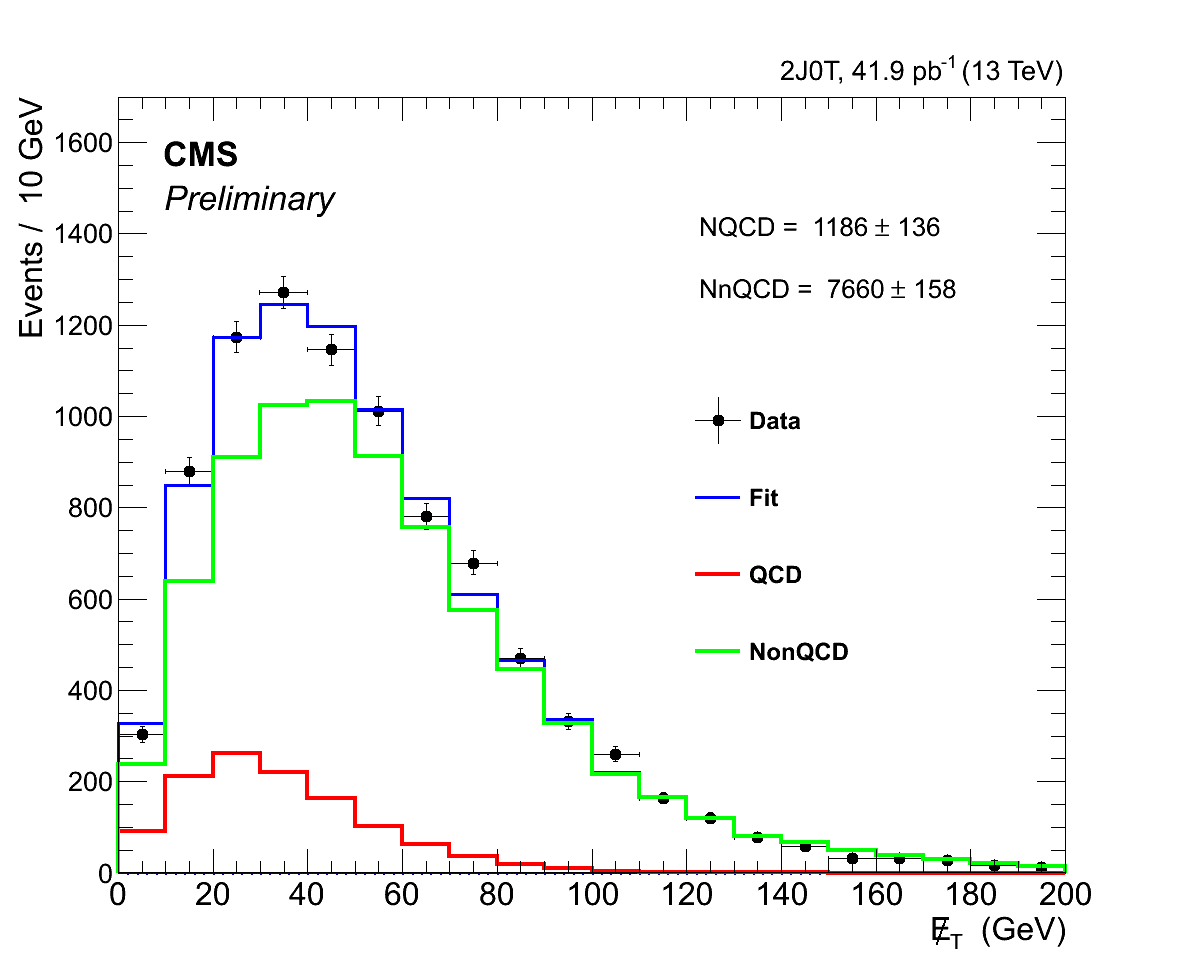
\includegraphics[width=0.45\textwidth]{figures/2J0T/Sep3/BinnedFit_MET_QCD_MC.png}
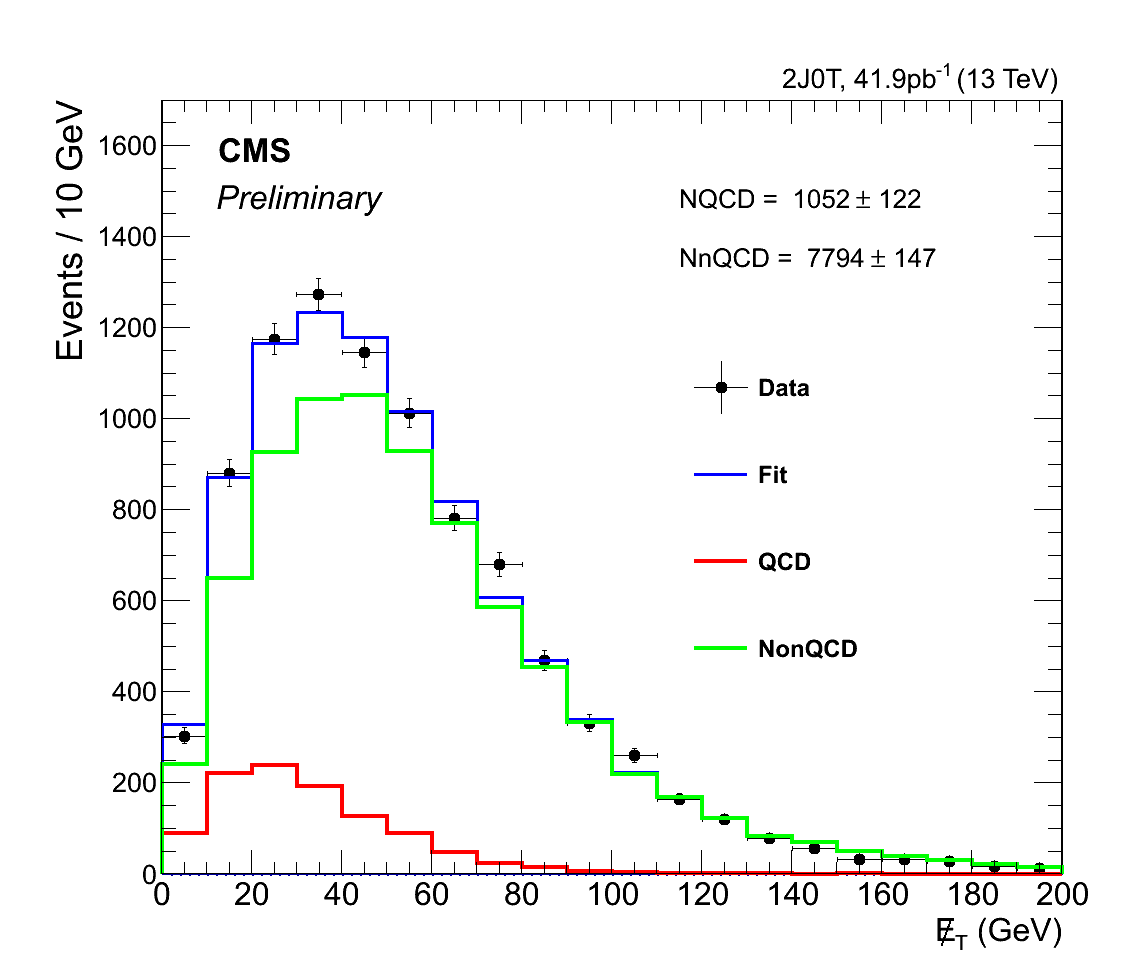
\includegraphics[width=0.45\textwidth]{figures/2J0T/Sep3/BinnedFit_MET_QCD_DD.png}\hfill
\caption{\label{fig:qcdFit3}Post fit distribution of $\met$ for binned fit where QCD shape is taken from MC (left) and data-driven (right)}
\end{center}
\end{figure}

\begin{table}[h]
\begin{center}
\caption{QCD estimation in the 2J0T region using $\met$}
\label{tab:QCDFitSF2}
\begin{tabular}{|c|c|c|c|c|c|}
\hline
Variable & Fit Type & QCD shape & Process & Fitted Yield & Extrapolated Yield\\
 & & & & (full range) & ($\met>45$GeV) \\
\hline
\multirow{4}{*}{\met} & \multirow{4}{*}{Binned}& \multirow{2}{*}{From MC} & QCD & 1186$\pm$136 & 319$\pm$37 \\\cline{4-6}
 & & & nonQCD & 7660$\pm$158 & 4330$\pm$89 \\\cline{3-6}
 & & \multirow{2}{*}{Data Driven} & QCD & 1052$\pm$122 & 248$\pm$29 \\\cline{4-6}
 & & & nonQCD & 7794$\pm$147 & 4405$\pm$83 \\\cline{3-6}
\hline
\end{tabular}
\end{center}
\end{table}
%\newpage
Significant difference between the results in section~\ref{sec:qcd2J0T} and $\met$-fit prompted us to investigated further. Upon investigation, significant mis-match in $\met$-templates for QCD
from MC and data-driven cases is observed. Also, mismatch between the MC and data-driven case in the distribution of $|\Delta\phi|$ between the muon and $\met$ in the transverse plane, has been
found out. But no such mismatch was seen in the muon p$_{T}$ and $\mT$ distributions. A positive corelation between $\met$ and $|\Delta\phi|$ is seen. 
We attribute this inconsistency to the incorrect estimation of $\met$ in data due to mis-identification of jets in high pseudorapidity region. Figures ~\ref{fig:MET_dphi} to ~\ref{fig:dphi_MET} summarize
the situation.
\begin{figure}[hbpt]                                                                                                                                                                            
\begin{center}
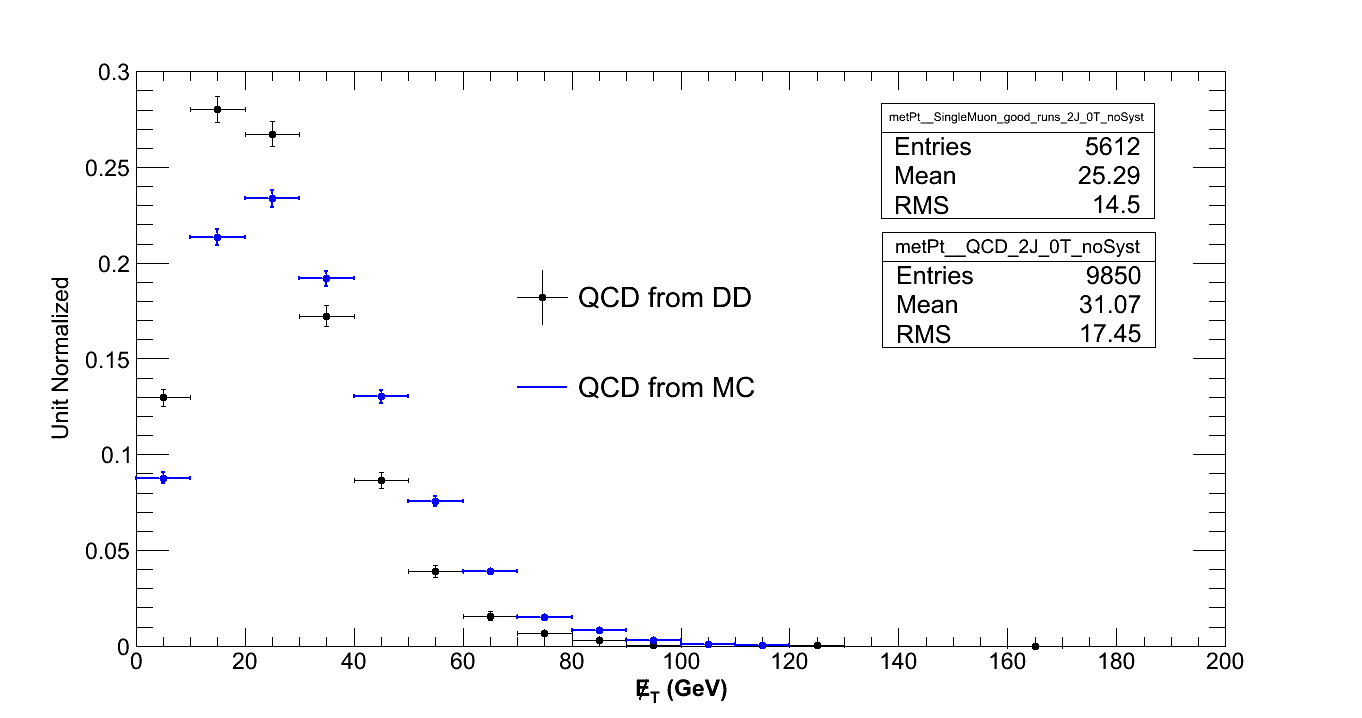
\includegraphics[width=0.45\textwidth]{figures/2J0T/QCD_Shape_Comparison_MET.png}
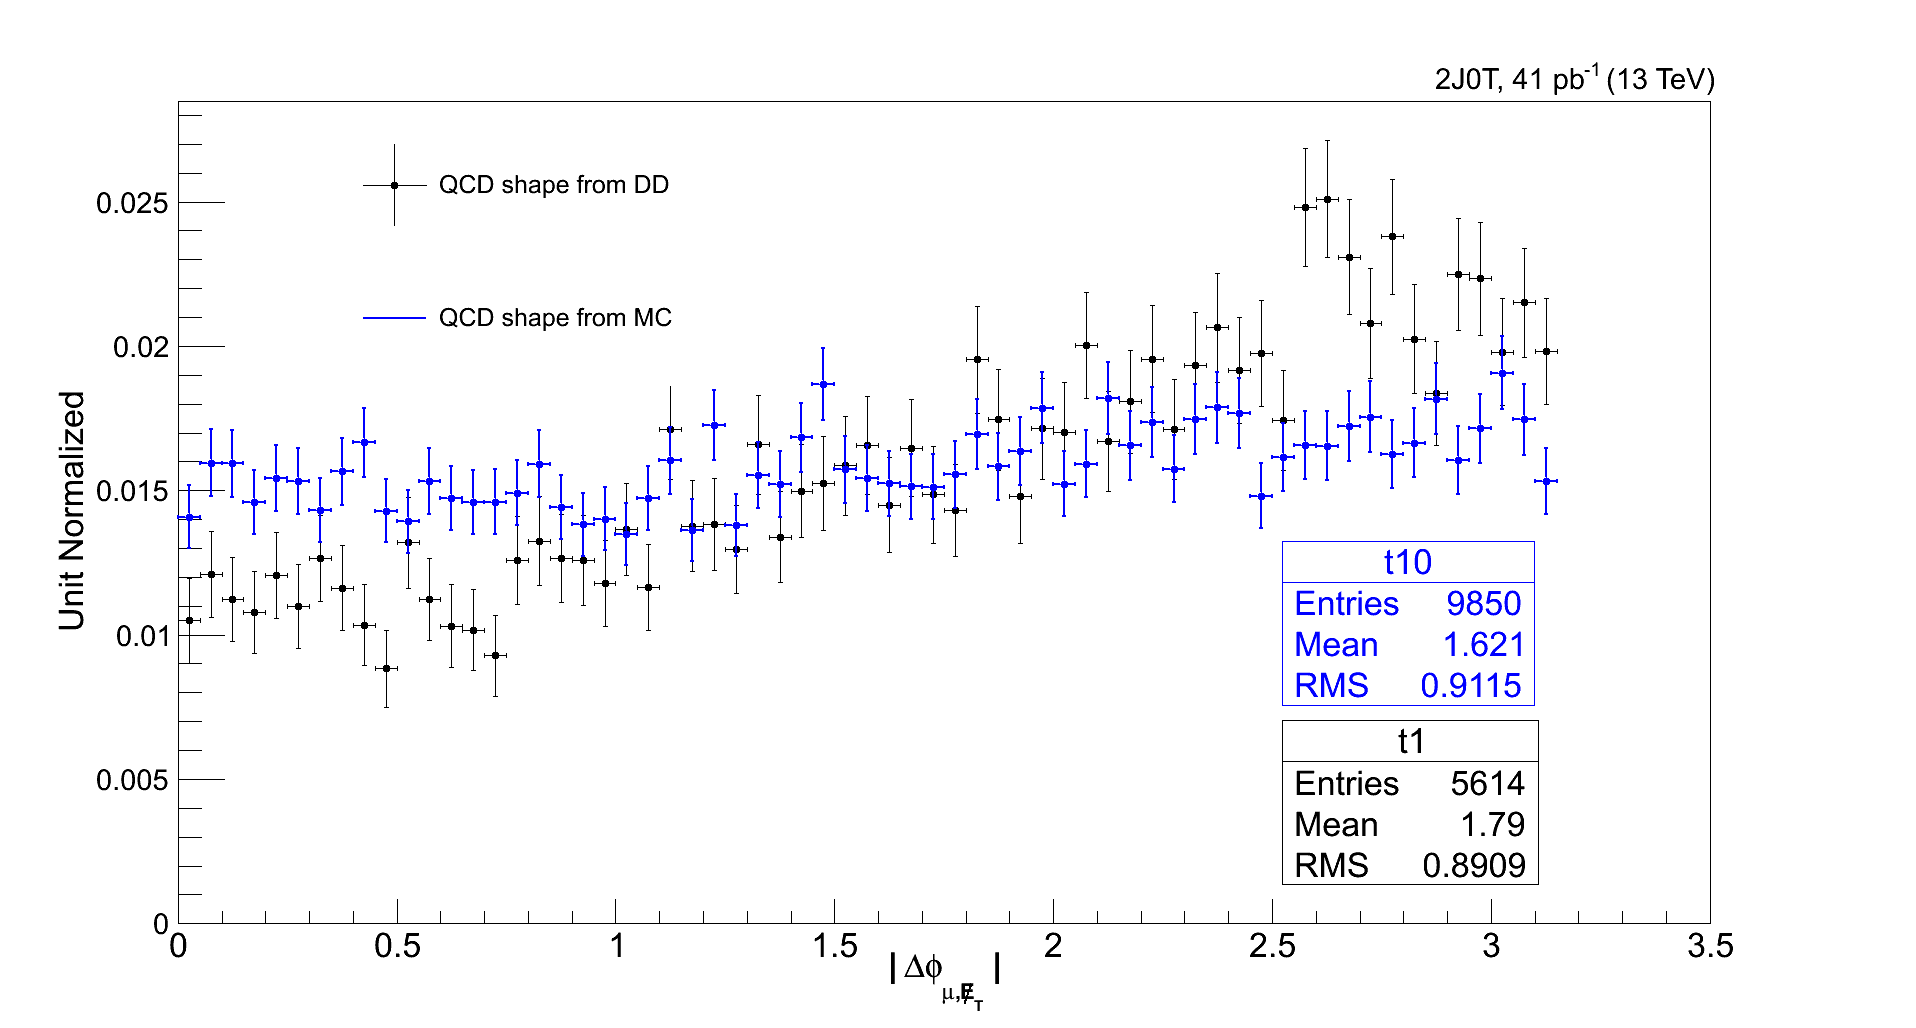
\includegraphics[width=0.45\textwidth]{figures/2J0T/QCD_MCvsDD_shapeComparison_dphi_muMET.png}\hfill
\caption{\label{fig:MET_dphi}Shape comparison of muon$p_{T}$ (left) and $\mT$(right) for QCD from MC and data-driven cases}
\end{center}
\end{figure}

\begin{figure}[hbpt]                                                                                                                                                                            
\begin{center}
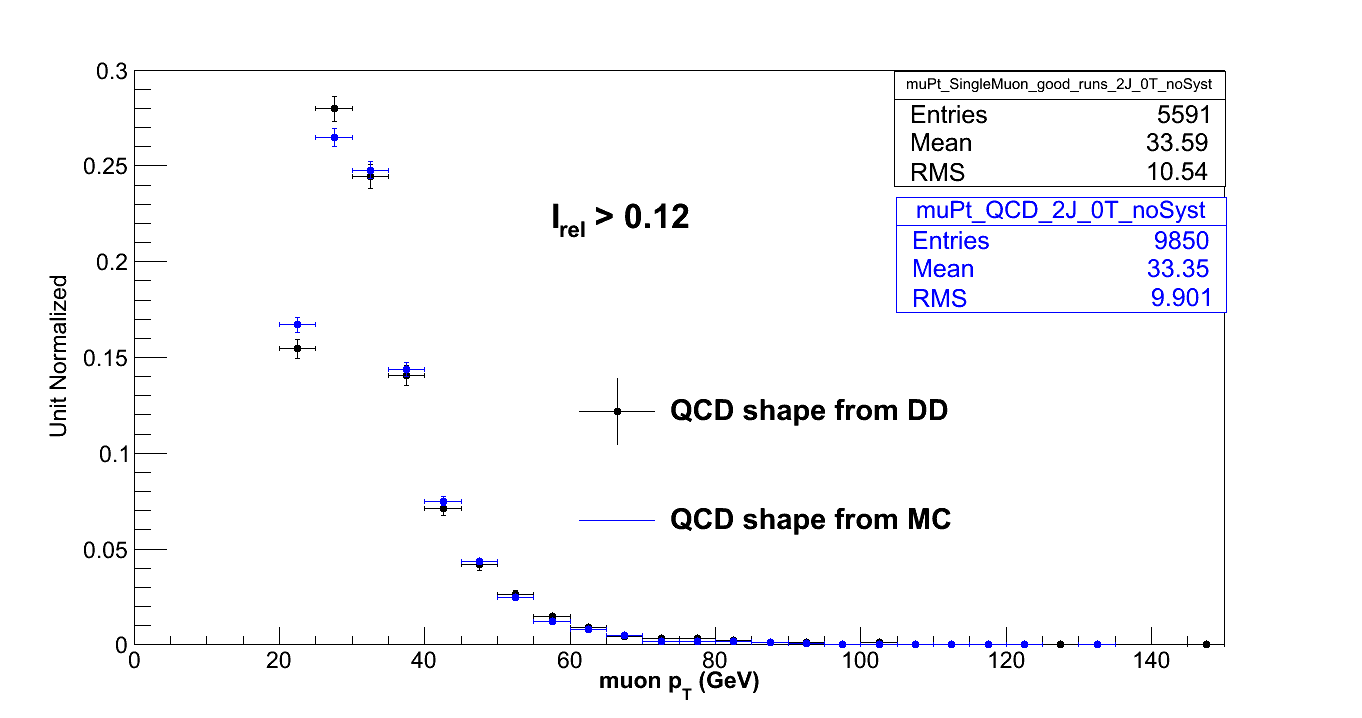
\includegraphics[width=0.45\textwidth]{figures/2J0T/QCD_Shape_Comparison_muPt.png}
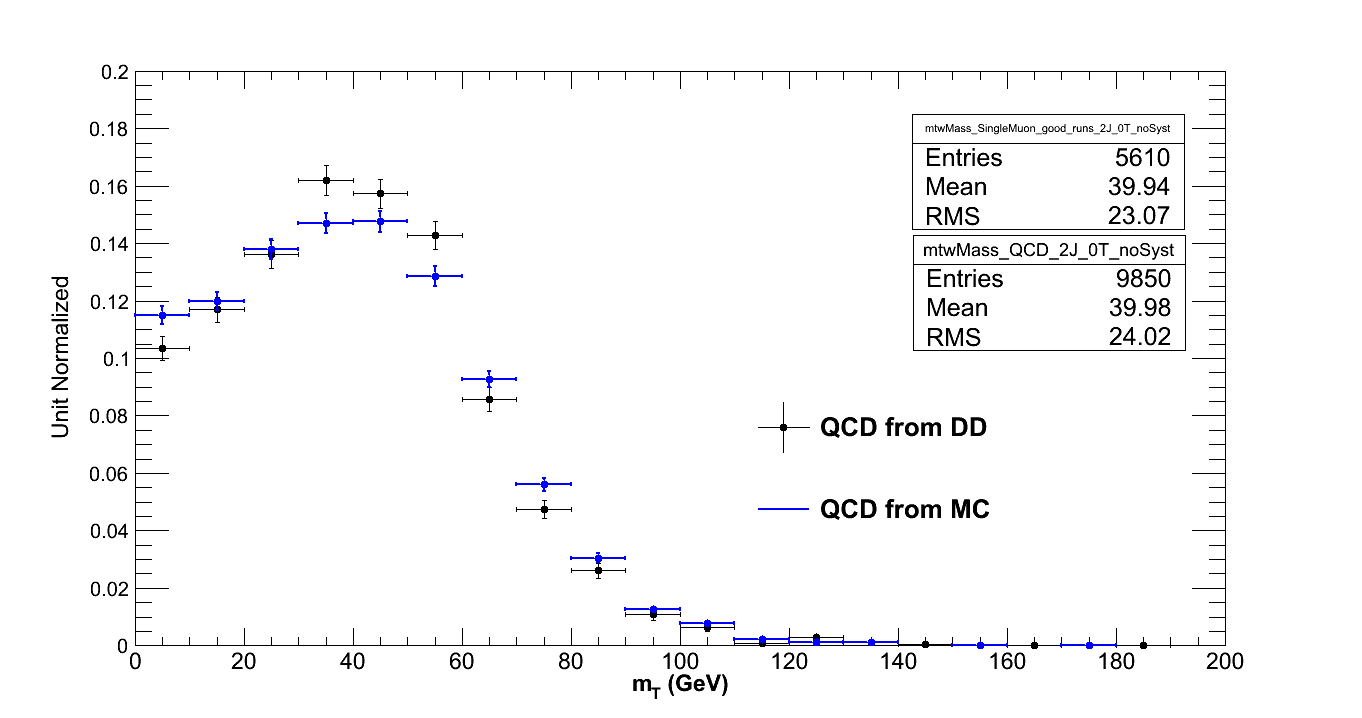
\includegraphics[width=0.45\textwidth]{figures/2J0T/QCD_Shape_Comparison_MtW.png}\hfill
\caption{\label{fig:muPt_mT}Shape comparison of muon$p_{T}$ (left) and $\mT$(right) for QCD from MC and data-driven cases}
\end{center}
\end{figure}

\begin{figure}[hbpt]                                                                                                                                                                            
\begin{center}
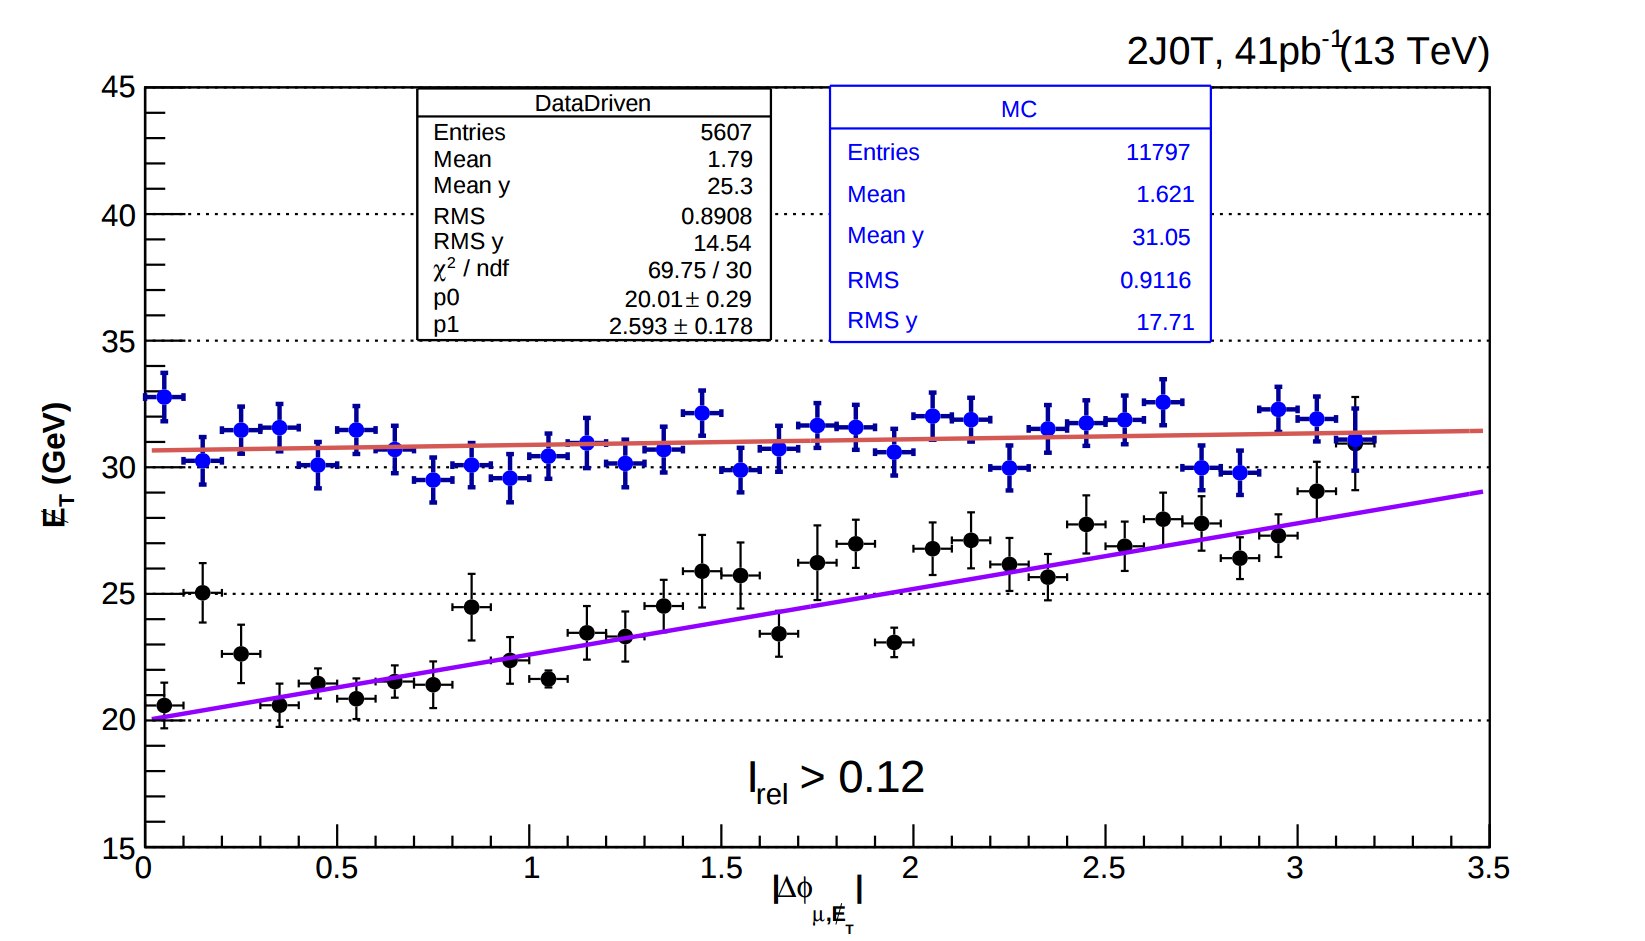
\includegraphics[width=0.65\textwidth]{figures/2J0T/MET_vs_dphimuMET.png}
%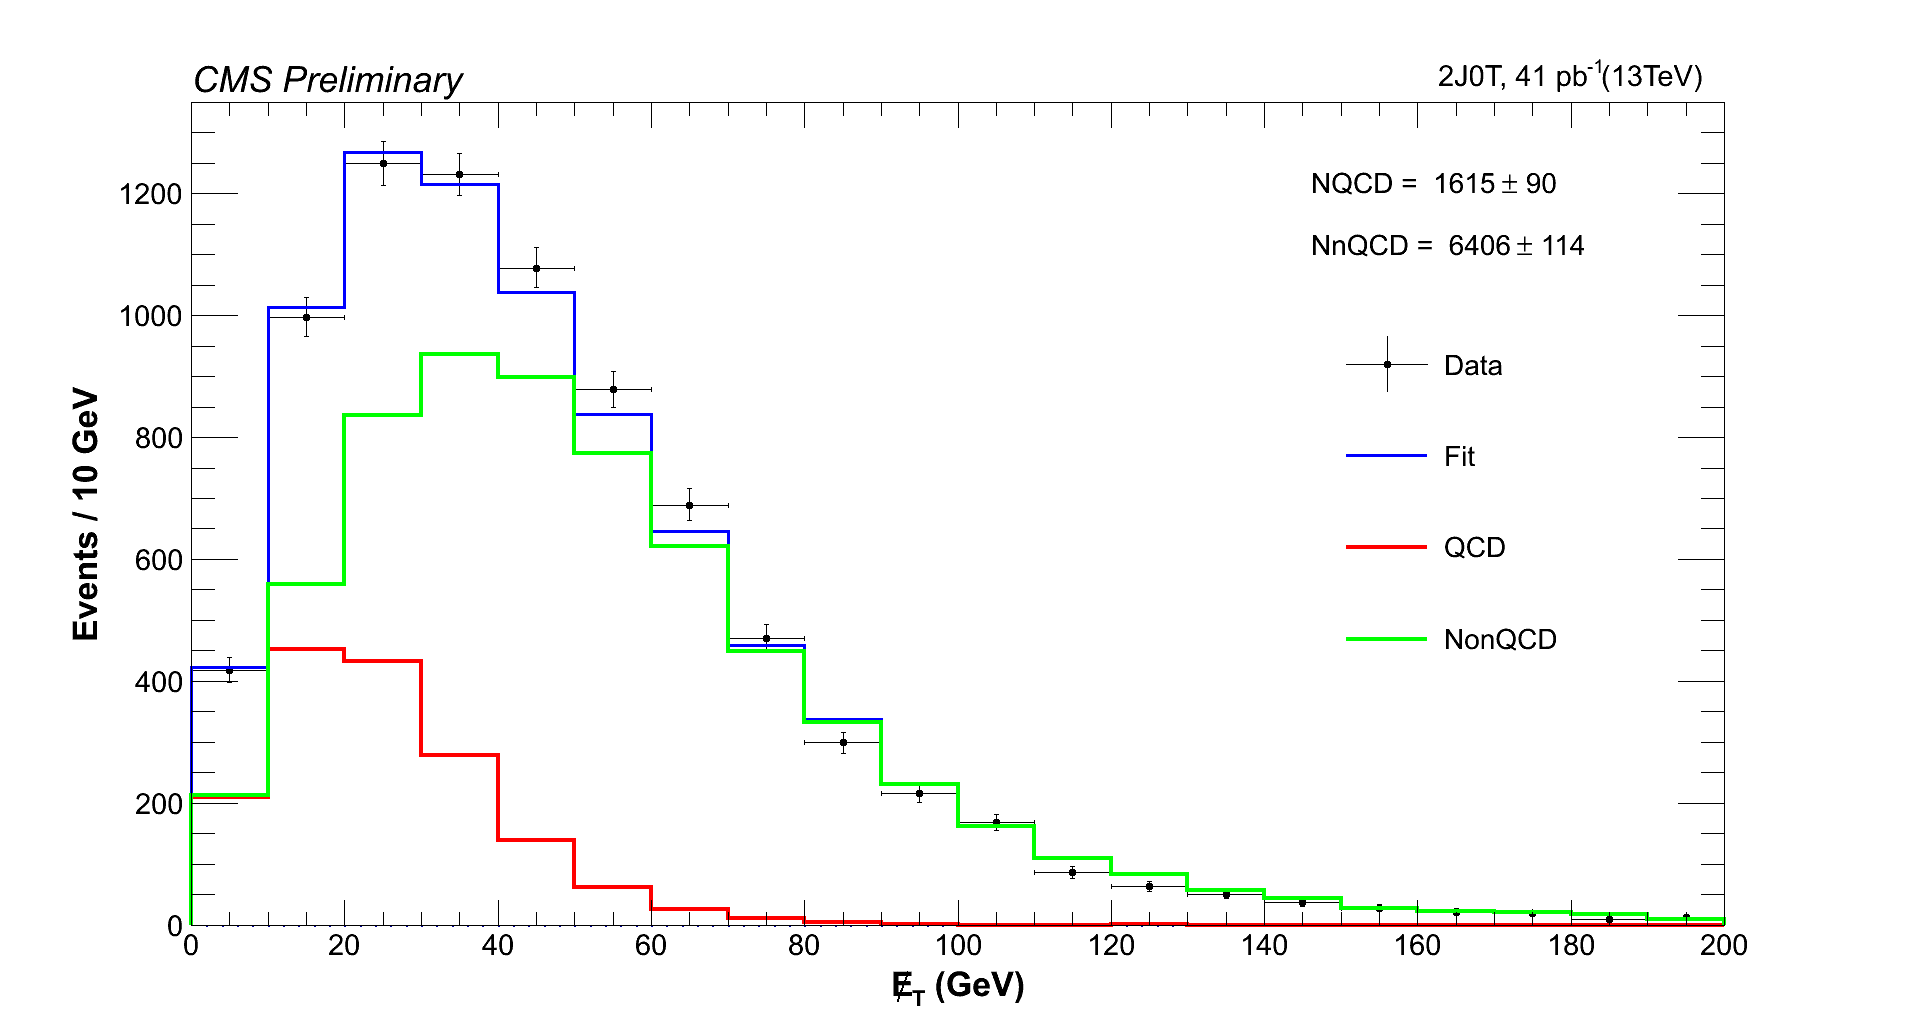
\includegraphics[width=0.45\textwidth]{figures/2J0T/Data_BinnedFit_MET_QCD_DD.png}\hfill
\caption{\label{fig:dphi_MET} Corelation between $\met$ and $|\Delta\phi|$ for MC and data-driven cases}
\end{center}
\end{figure} 
